%about objects not information; we can discuss in outside the box the issue of
%information needed forver but shuttled in and out.

\chapter{Extreme Scalability of Long-lived Data}
\label{chapter:large-long-lived}

All of the tuning advice presented so far in this book can only get you so far.
Sometimes, despite your best efforst of tuning entities and collections, your
application's objects still do not fit into the memory constraints of the target
platform. Managing a great number of long-lived objects therefore comes with its
own set of challenges, even though objects these objects are free from the bugs
that riddle those with correlated lifetime. To manage objects that, after a
reasonable amount of tuning, still don't fit into the heap, you have three
solutions at your disposal: throw hardware at the problem, implement a kind of
demand paging, or code your data models in a non-object oriented way.

\paragraph{Buy More Memory} The first solution you may consider is buying more
memory for the target platform. If your budget allows for this, then by all means
you should strongly consider doing so. There are some downsides to keep in mind.
The first is heap size limits. At some point, you will need to switch from a
32-bit JVM to a 64-bit JVM\index{64-bit}. This switch will result in a large
increase in overhead. As discussed earlier, the amount of blowup resulting from a
switch to a 64-bit JVM depends on the degree of delegation in your data models. A
64-bit JVM only adds overhead to the extent that your data models have headers
and pointers. The alternative, running with compressed
references\index{Compressed References}, limits you to around 32GB of memory, and
imposes a few percent slowdown. In addition, running with a large heap can result
in increases in the length and fluctuations in pause times.

\paragraph{Shuttle Objects in and Out of the Java Heap} Rather than attempting to
fit all of your objects into a single heap, you can store them outside of the
Java heap, and swap them in (and out), on demand. If the logic of your
application allows for recomputing the data stored in these objects, you need to
be careful to compare the recreation cost with the costs of marshalling objects.
You can choose to marshall objects to and from a local disk, or you can use one
of several frameworks that provide a distributed key-value map.

\paragraph{Break the Java Mold} Despite being an object-oriented language, there
is nothing in the Java language that prevents you from storing objects in a
non-object oriented way --- nothing, that is, except programming time and
maintenance expense. It is possible to store data only in arrays, as one would in
a language such as Fortran, and retain a great deal of object orientation in your
data models and programming interfaces. 

This chapter presents a methodology for predicting the scalability of your data
models, and presents several solutions to demand-marshalling objects, and for
storing objects in a ``Fortran style''.

\section{Scalability: Quantitative Methodology}

\begin{figure}
\centering
	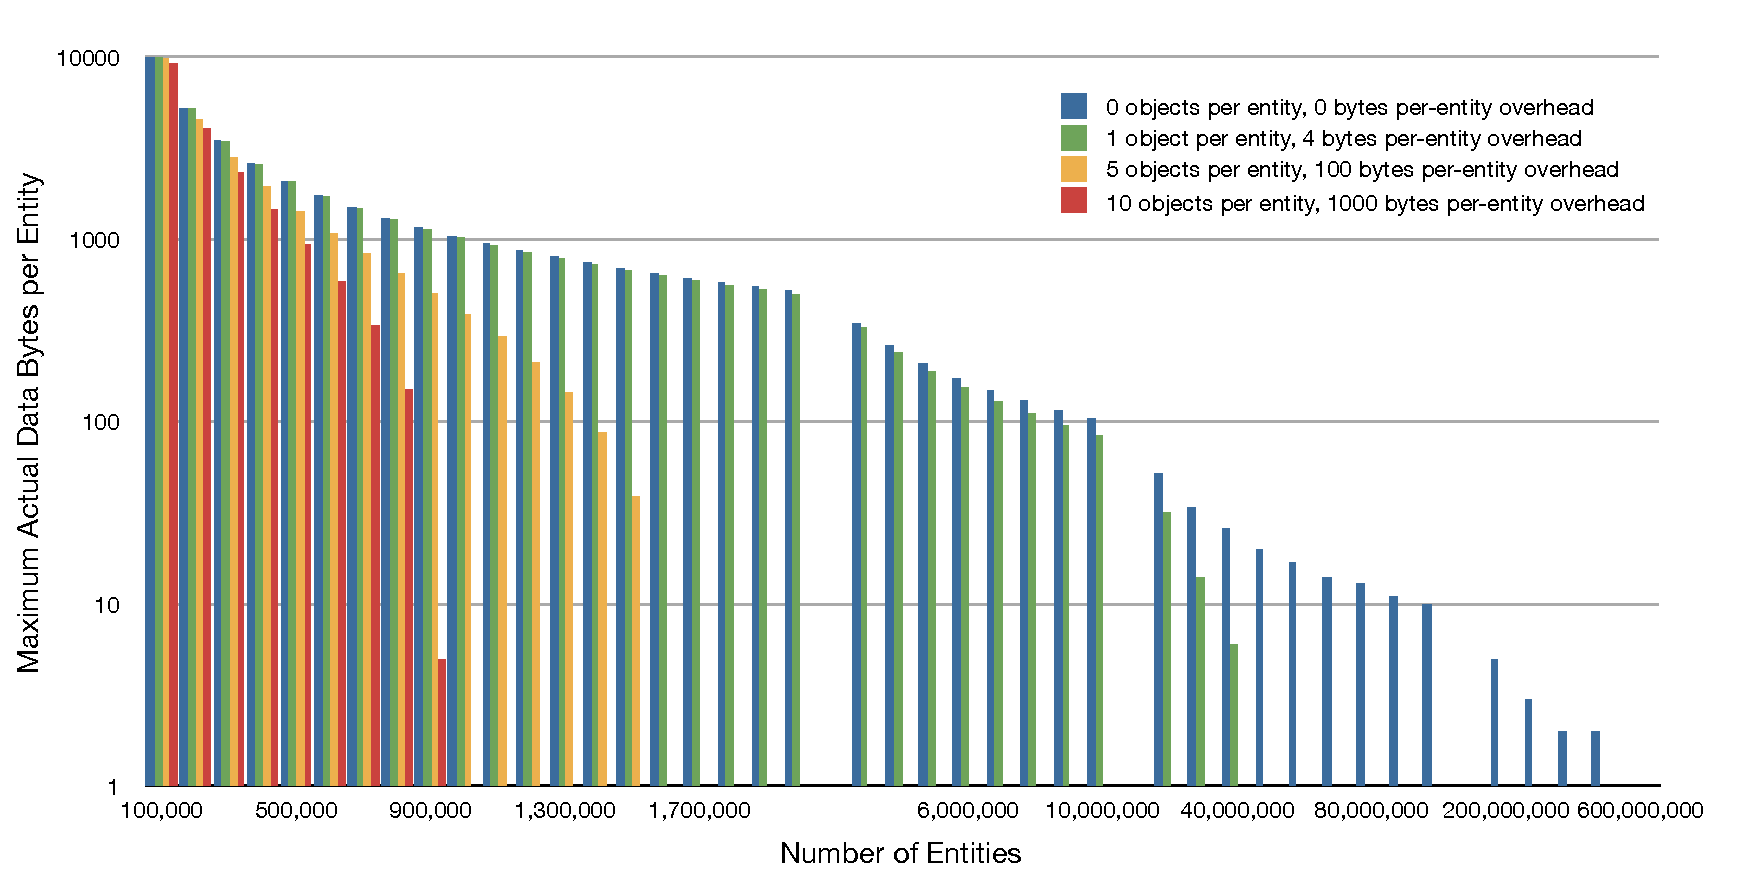
\includegraphics[width=\textwidth]{part4/Figures/maxActualData}
	\caption{The amount of actual data you can store in your entities depends on
	the degree of delegation in your entities, and the per-entry overhead of the collection in which these entities
	reside. This chart assumes a limit of 1 gigabyte of Java heap.}
	\label{fig:maxActualData}
\end{figure}

TODO: write this section, explaining \autoref{fig:maxActualData}.

\section{Representing Relationships}

When representing relationships between entities, using standard object oriented
practices, you are severely limited in the number of entities and relationships
that you can store. Doing so in a straightforward manner, one that obeys object
oriented practices, is very similar to the task of representing a graph of nodes
and edges. For example, when caching data from a relational database in the Java
heap, the entities (rows in a database table) and relations (columns that contain
indices into tables) become the nodes and edges in a graph.

%\begin{example}{Storing a Graph}
If a graph has a great many nodes and edges, you must design its storage
carefully. Consider the small example illustrated in 
\autoref{fig:exampleGraph}. There are several ways to implement the abstract
data types, of nodes and edges, shown in that figure. Each strategy has its
positives and negatives, depending on whether ease of maintenance or memory
consumption are of primary importance.
%\end{example}

\begin{figure}
\centering
\subfigure[Example graph.]{
\shortstack{
	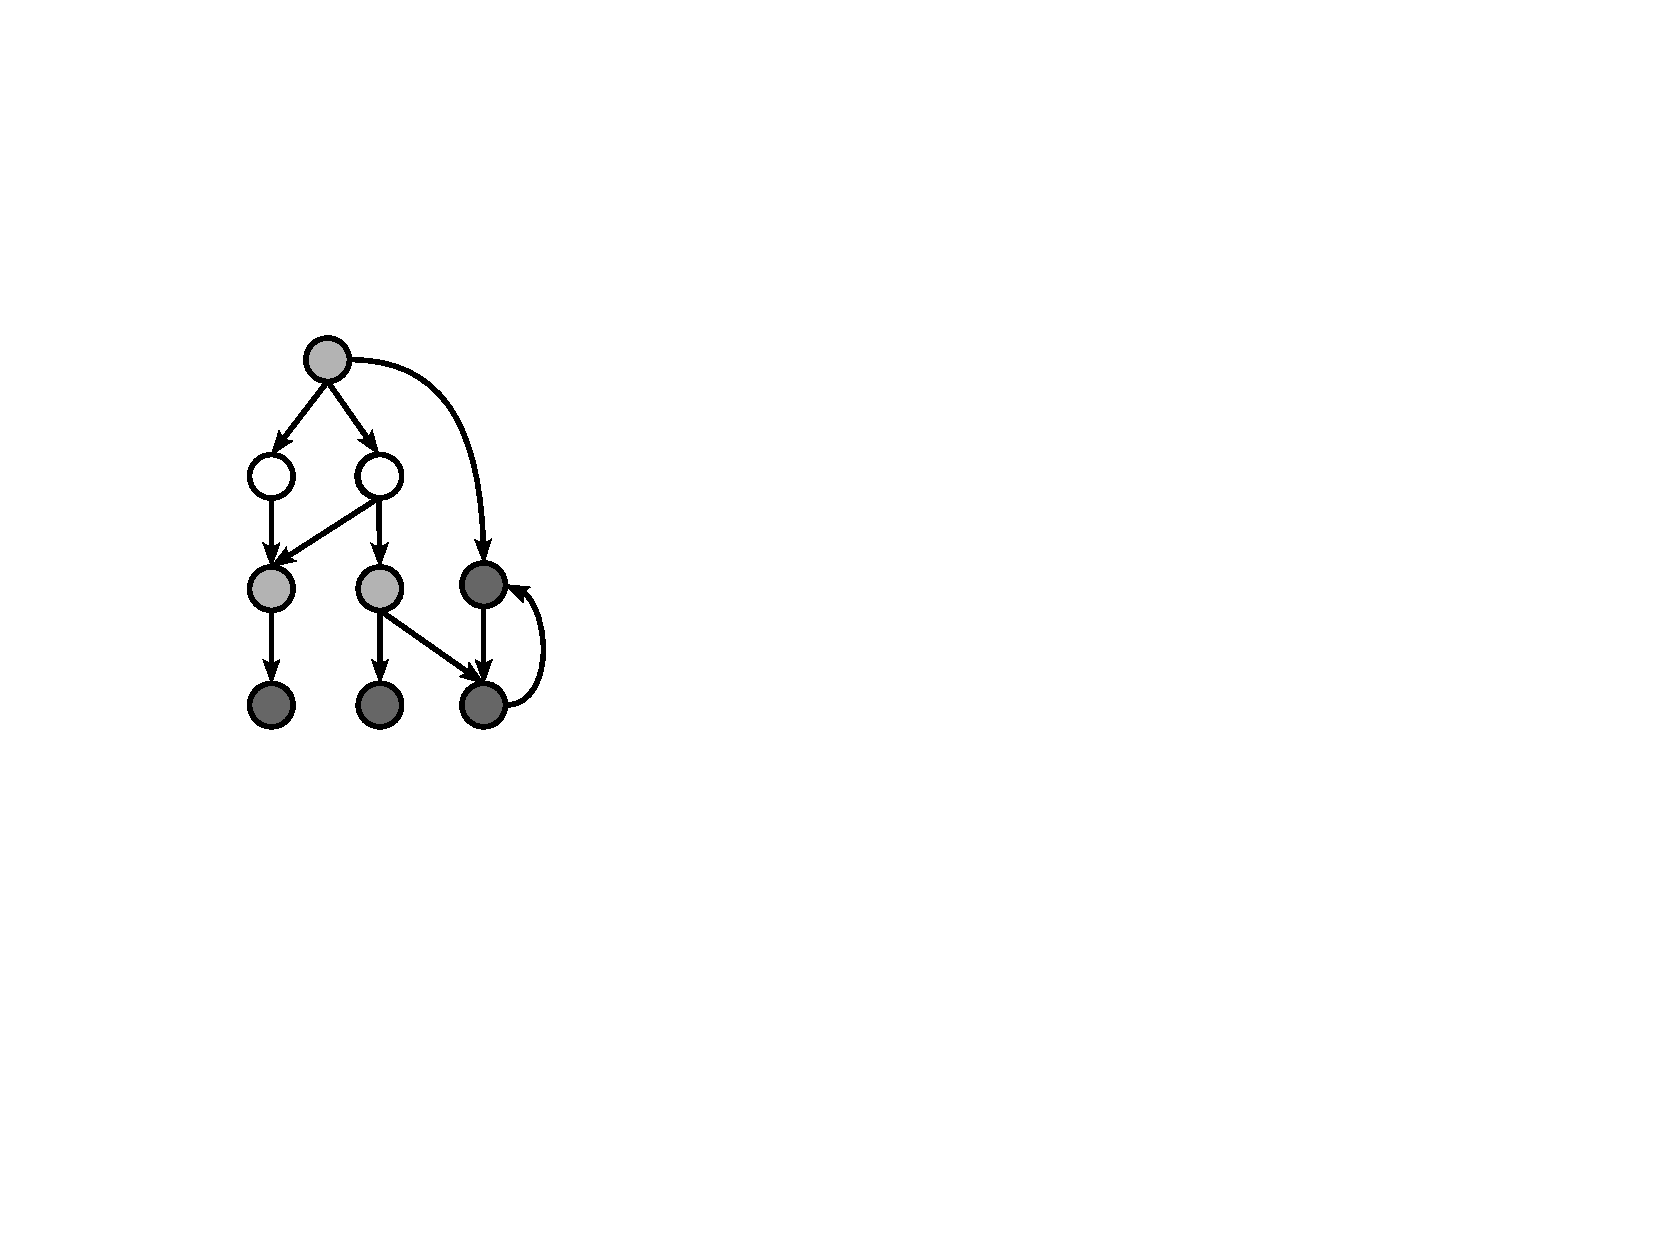
\includegraphics[width=0.3\textwidth]{part4/Figures/exampleGraph}
	\\ \vspace{5mm}
	}
}
\begin{subfloat}
\label{fig:graph-interfaces}
\begin{minipage}[b]{0.65\textwidth}
\begin{shortlisting}
interface Graph {
	Set<Node> getNodes();
	Set<Edge> getEdges();
}
interface Node {
	Color getColor();
	List<Edge> getChildren();
	List<Edge> getParents();
}
interface Edge {
	Node getFrom();
	Node getTo();
}
enum Color {
	White, LightGray, DarkGray
}
\end{shortlisting}
\end{minipage}
\caption{Abstract data types for nodes and edges.}
\end{subfloat}
	\caption{An example generic graph of three colors of nodes.}
	\label{fig:exampleGraph}
\end{figure}

\begin{figure}
\centering
\begin{subfloat}
\begin{minipage}[b]{0.44\textwidth}
\begin{shortlisting}
class Node {
   Color color;
   List<Edge> parent;
   List<Edge> child1;
   List<Edge> child2;
}
\end{shortlisting}
\end{minipage}
\caption{Concrete classes}
\end{subfloat}
\begin{subfloat}
\begin{minipage}[b]{0.568\textwidth}
\begin{shortlisting}
public Node(Color color) {
   color = color;
   parents = new ArrayList();
   children = new ArrayList();
}
\end{shortlisting}
\end{minipage}
\caption{Node constructor that uses the default \class{ArrayList} constructor.}
\label{fig:node-obvious-constructor}
\end{subfloat}
\caption{A straightforward implementation of the Node interface.}
\label{fig:node-obvious-impl}
\end{figure}

\autoref{fig:graph-interfaces} shows the interfaces for a \class{Graph},
\class{Node}, and \class{Edge} that one must implement. A common implementation
strategy, applied to the \class{Node} and \class{Edge} data types, is a
straightforward mapping of interfaces to concrete classes.
\autoref{fig:node-obvious-impl} shows such an implementation for the
\class{Node} data type. Following this
strategy, the \class{Node} class has three fields, to store its \class{Color}
and the relations to children and parents; these relations are implemented with a
standard collection, likely an \class{ArrayList}. The \class{Edge} class has two
fields, to store pointers to the source and target nodes. This implementation is
easy to implement. It is also easy to maintain: changes to the interfaces can be
directly mapped to changes to the implementation, because the two are parallel
versions of each other. The nodes and edges, and relations between them, are
objects that can be manipulated using normal object oriented practices; e.g. you
can write \texttt{node.getChildren().get(5).getTo()\-.getColor()}, which reads
as a fairly natural, albeit verbose, expression of what you intend.

\paragraph{A Straightforward Implementation}
Without any thought for memory concerns, the constructor for a node would be as
shown in \autoref{fig:node-obvious-constructor}. In this implementation, the
memory cost per node is three pointers plus two collections of default size. As
\autoref{tab:collection-costs} shows, the the default constructor of an
\class{ArrayList} allocates an array to hold 10 elements; the per-collection cost
is 80 bytes and the per-entry cost is 4 bytes. If no node has more than 10
parents or 10 children, then each node will consume one object header plus $3*4 +
2*(80 + 10*4)$, or $264$ bytes. If, on average, a node has one parent and 2
children, then 68 bytes (27\%) of this cost is wasted on null pointers. The 80
bytes (31\%) spent on the parent collection is unnecessary, for those nodes that
have exactly one parent. Even an optimally structured list which includes just
one pointer for a list with one entry would still impose two pointer costs to
reference a single parent node (one pointer to reference the list, one for the
list to reference the parent node).

In addition to the cost of the nodes are the cost of the edges objects. By
objectifying each edge, this implementation pays a cost of one object header
plus two pointers, or 24 bytes (20 bytes, before rounding up to an 8-byte
alignment boundary). For the example with an average of one parent and two
children per node, the effective cost per node is $264 + 3*24$, or $336$ bytes.

Ideally, a node with one parent and two children should consume four pointers, or
16 bytes: one to reference a \class{Color}, one to reference the parent node, and
two pointers to reference the children. The disparity between this optimal value
and the cost of the standard implementation is 320 bytes. A inspection
of \autoref{fig:maxActualData} shows that this implementation, with 16 bytes of
actual data and 320 bytes of overhead, can support at most 2.7 million
nodes per gigabyte of heap. An ideal implementation, with no storage costs
beyond the necessary 16 bytes of pointers, would be able to support 65
million nodes per gigabyte of heap.

\paragraph{Optimizing the Implementation}
By specializing your code to handle only a limited degree of functionality, you
can achieve a fair degree of compactness without much effort. If every node has
exactly the same number of incoming and outgoing edges, an easy alternative
implementation presents itself. You can specialize the implementation for this
structural special case, and thereby eliminate the waste that comes from allowing
a flexible number of incident edges.
\autoref{fig:node-tuned-impls}a shows an implementation of the \class{Node}
interface that does away with collections. On top of the ideal implementation,
the cost per node is one object header plus two pointers for each of the three
\class{Edge} objects. On top of the 16 byte ideal cost, this implementation costs
an additional $3*(2*12 + 2*4)$ bytes, for a total of 112 bytes. This cost is
1/3rd the cost of the initial implementation, though 7 times that of the ideal
implementation. This implementation supports just over 9 million nodes per
gigabyte of heap.

Even if many nodes have no parents, or fewer than two children, this specialized
implementation remains preferable to the original one that uses collections. This
is because an empty collection consumes no less than then the one pointer that
this collection-free implementation costs; this is the case if you point to the
singleton \code{Collections.emptyList()}. In the case when a node has one child,
then a list must be allocated, whose expense, even if the list has only a single
entry, will always be higher than a single pointer.

\begin{figure}
\centering
\begin{subfloat}
\begin{minipage}[b]{0.38\textwidth}
\begin{shortlisting}
class Node {
   Color color;
   Edge parent;
   Edge child1;
   Edge child2;
}
\end{shortlisting}
\end{minipage}
\label{fig:node-no-collections}
\caption{No collections}
\end{subfloat}
\qquad
\begin{subfloat}
\begin{minipage}[b]{0.38\textwidth}
\begin{shortlisting}
class Node {
   Color color;
   Node parent;
   Node child1;
   Node child2;
}
\end{shortlisting} 
\end{minipage}
\caption{No objectified Edges}
\label{fig:node-no-Edge-objects}
\end{subfloat}
\caption{Two implementations that have been specialized for the case where
no object has more than one parent and no more than two children.}
\label{fig:node-tuned-impls}
\end{figure} 

\autoref{fig:node-tuned-impls}b shows a yet more highly optimized \class{Node}
implementation that stores pointers to \class{Node}s, rather than \class{Edge}s.
One somewhat extreme variant of this implementation does not store \class{Edge}
objects at all. This \class{Edge}-free implementation approaches the ideal
implementation, in its capacity for storing large graphs. You must still pay one
object header per node, for the \class{Node} objects themselves. Thus, this
impementation has a per-node memory cost of 16 bytes for the pointers plus 12
bytes for the header. At this unit cost, a one gigabyte heap would support 37
million nodes.

Though quite scalable, this implementation presents several complications.
First, if the API specifies that \code{Node.getChildren()} returns a list of
edges, then an \class{Edge}-free storage strategy must return facades that route
the edge operations properly. The same issue holds for an implementation that
stores only a single parent pointer: how can one efficiently support an
interface that expects a list of edges, if the storage contains only a single
pointer? The following implementation does not work:

\begin{shortlisting}
public List<Edge> getParent() {
   List<Edge> list = new ArrayList<Edge>();
   list.add(parent);
   return list;
}
\end{shortlisting}

In addition to being quite expensive, in creating a list for every call to
\code{getParent}

lacks
in expressive power compared to the other implementations presented so far. For example you will find it more
difficult to extend the graph interface to support edge labels. Doing so is not
impossible, of course, but requires some careful planning, and thinking outside
the Java box.

\paragraph{Supporting Edge Properties in Optimized Implementations}

You may choose to store the edges in a side data structure, such as a map.
However, except in the case where , but this will not have much benefit


If \class{Node.getChildren()} returns a list of nodes, rather than a list of
edges, then the code to access an edge label of the second child of a node can no
longer be \texttt{node.getChildren().\-get(1).getLabel()}. This way of traversing
the graph leads to a node, not an edge! If the API instead returns an
\class{Edge} You don't even have the option of implementing the edge
abstraction, under the covers. That is, you cannot both avoid storing \class{Edge} objects and yet support an external interface of
\class{Edge}s:

\begin{shortlisting}
public class Node {
   private Node parent; // field stores Node, not Edge
   public Edge getParent() { // API returns an Edge
      
   }
}
\end{shortlisting}

Instead, edge labels must be fetched from
the graph model itself, such as via \texttt{graph.getEdge(from, to).getLabel()}.

Furthermore, without some care, every edge label query will require a hash table
lookup.


Java, as it currently stands, makes certain access patterns difficult. Using a
fully object-oriented Java design, it is impossible to achieve both compactness
of storage and the generality to handle a variety of graph structures. To do so
requires coding in a style that is not conventionally object oriented.



 Shortly, we will discuss the
complexities, but benefits, of the latter style of API.




\section{Breaking the Mold of Object Orientation}
\label{sec:fortran-style}

\subsection{The Bulk Sharing Pool}
\label{sec:bulk-sharing-pool}

The bulk storage that backs a set of data items, each of the same type. Objects
share the data by indexing into the pool.

\subsection{Column-oriented Storage}
\label{sec:column-oriented}

\section{Memory Mapping and Marshalling}